\section{The McCreary Intelligent Textbook Corpus}\label{sec:corpus}

This section formally defines the corpus for the first time in literature.

\subsection{Corpus Description}\label{sec:corpus-desc}

The McCreary Intelligent Textbook Corpus comprises 25 open-source educational
textbooks hosted on GitHub (\url{https://github.com/dmccreary}). Each textbook
contains a standardized learning graph encoded as a CSV file representing a
directed acyclic graph (DAG) of concepts and their prerequisite dependencies.

The corpus spans three categories:
\begin{itemize}
  \item \textbf{STEM} (11 domains): calculus, biology, genetics, bioinformatics,
    statistics, quantum computing, circuits, geometry, ecology, moss, functions.
  \item \textbf{Professional} (7 domains): economics, organizational analytics,
    healthcare data modeling, database selection, conversational AI,
    automating instructional design, blockchain.
  \item \textbf{Foundational} (7 domains): systems thinking, theory of knowledge,
    digital citizenship, prompt engineering, AI tracking, US geography, ASL.
\end{itemize}

Key statistics:
\begin{itemize}
  \item Concepts per domain: 140--550 (mean: $\sim$267)
  \item Total concepts: 12,260
  \item Total edges: 19,405
  \item Taxonomy categories: 1--19 per domain
  \item Raw content: MkDocs Markdown chapters ($\sim$3,000--8,000 words per textbook)
\end{itemize}

Figure~\ref{fig:learning-graph} shows the interactive learning graph viewer
for the calculus domain, illustrating the DAG structure with color-coded
taxonomy categories and prerequisite edges.

\begin{figure}[htbp]
\centering
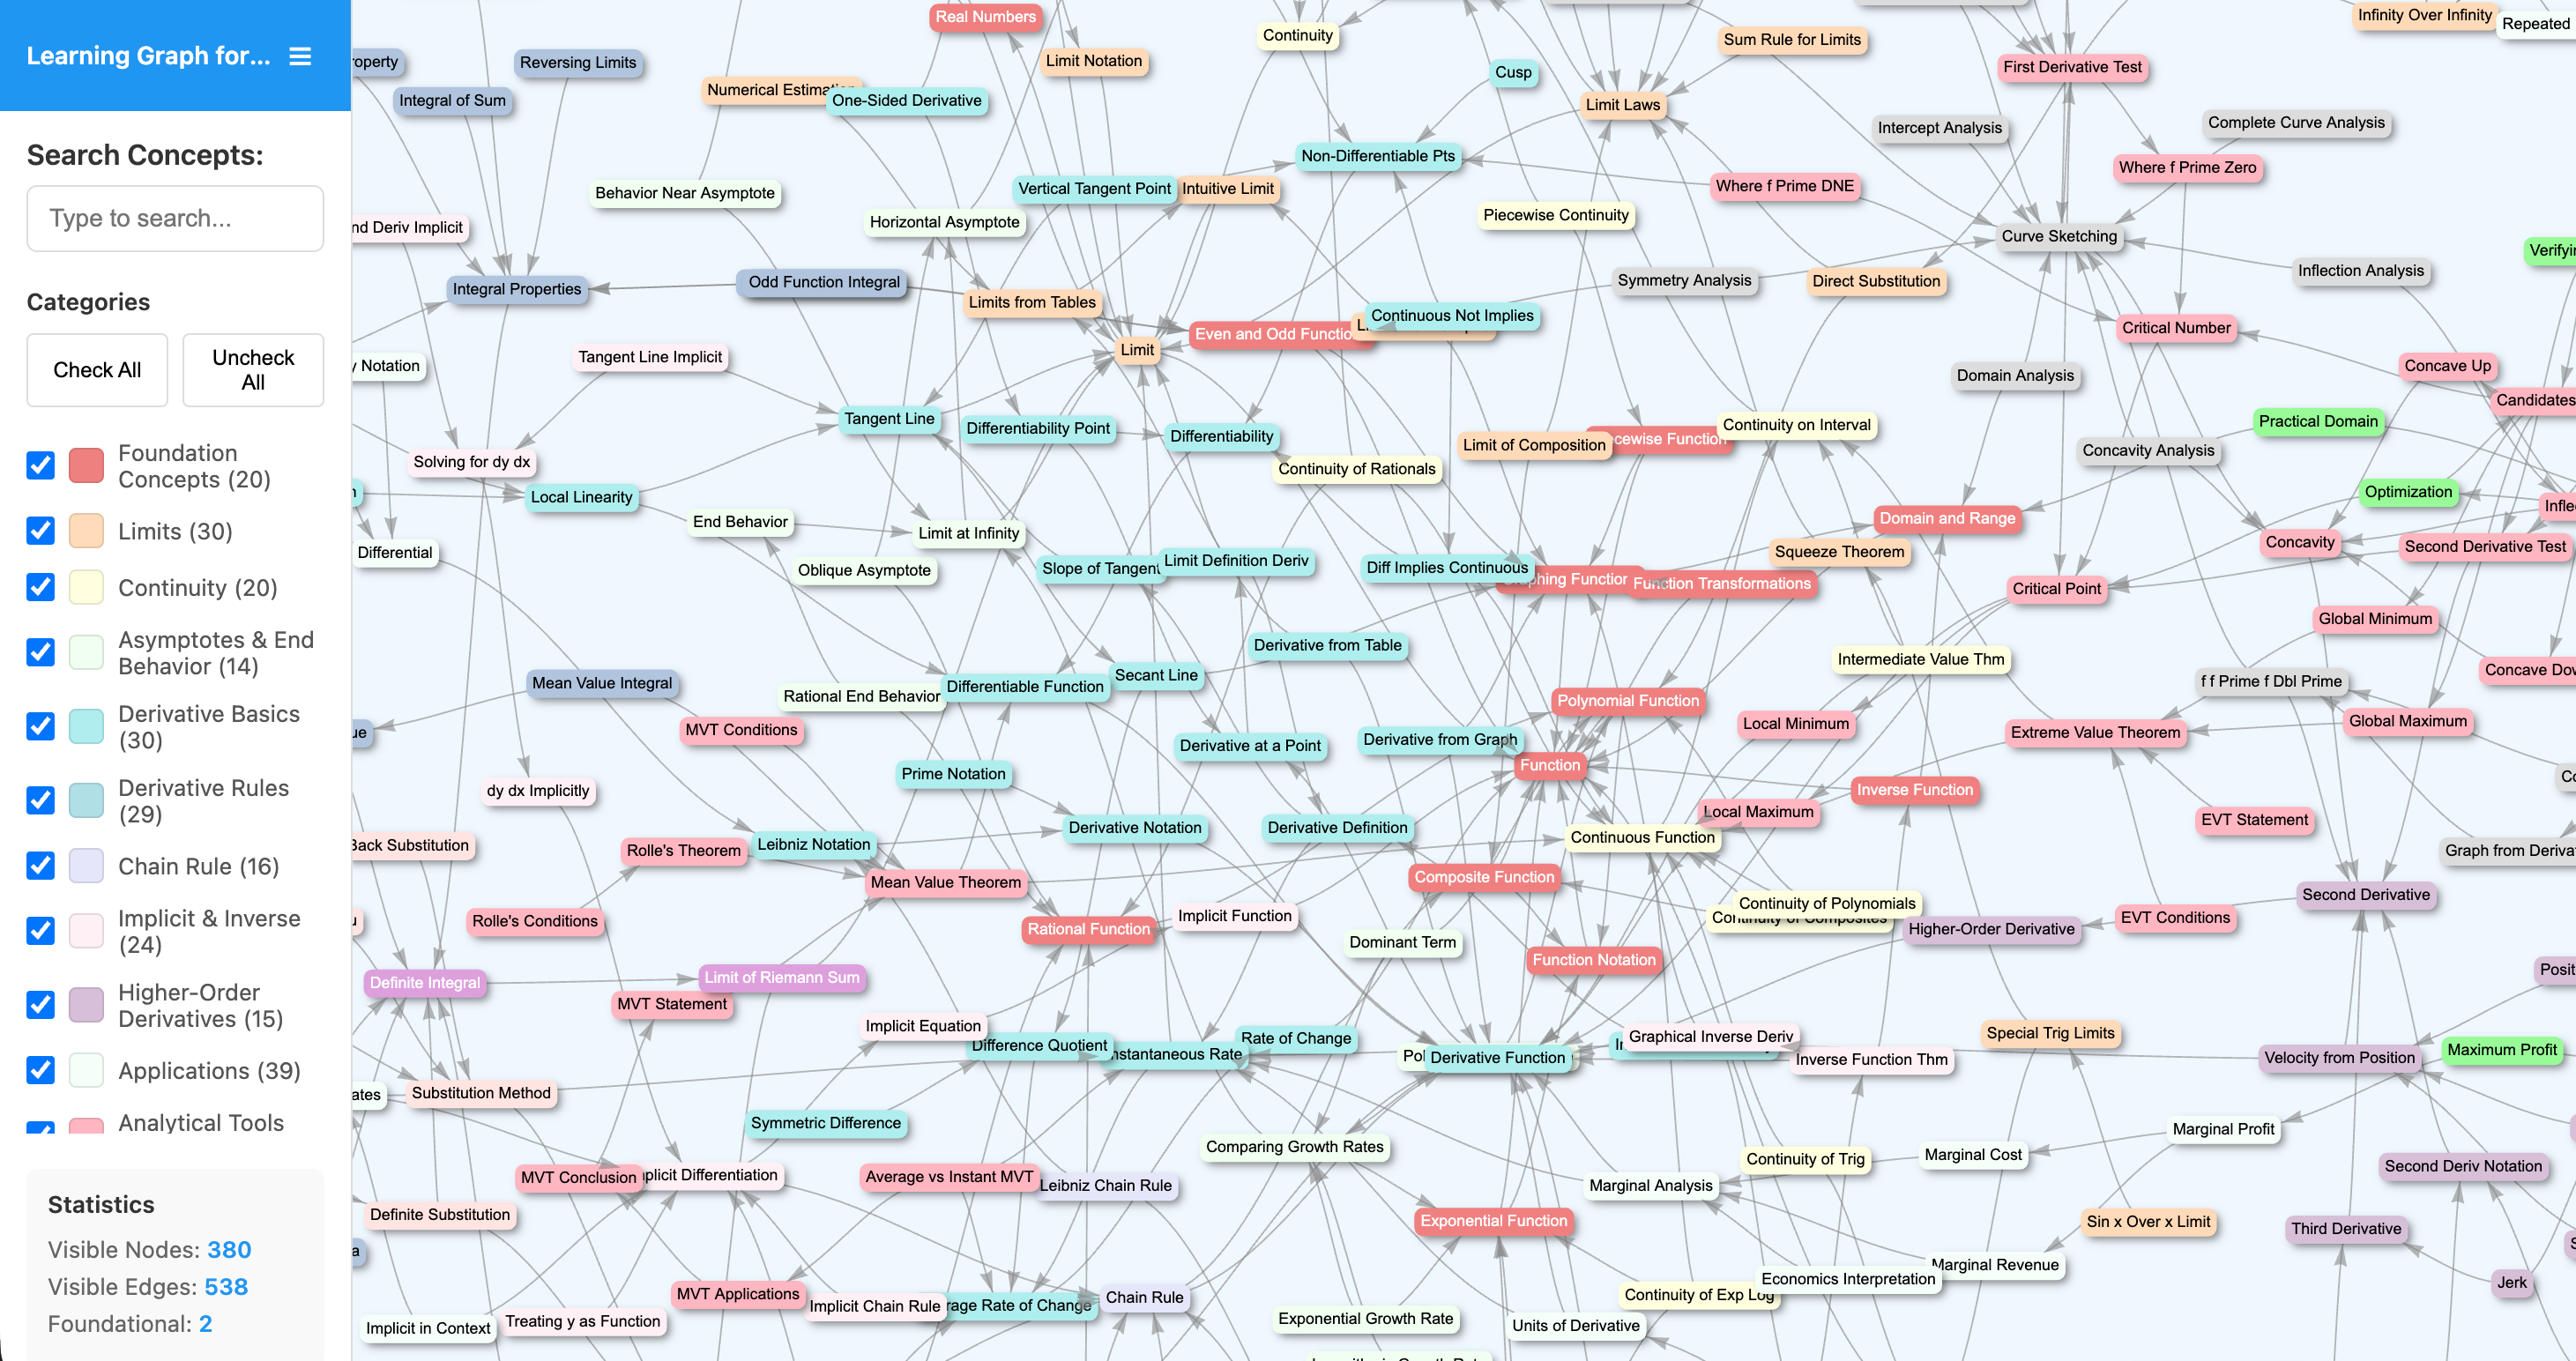
\includegraphics[width=0.95\textwidth]{figures/calculus-learning-graph.png}
\caption{Interactive learning graph viewer for the calculus domain (380 concepts,
539 edges). Each node is a concept, color-coded by taxonomy category. Directed
edges represent prerequisite dependencies. The left panel shows category filters
and corpus statistics. All 46 domains in the McCreary corpus use this same
DAG structure.}
\label{fig:learning-graph}
\end{figure}

\subsection{Corpus Schema}\label{sec:corpus-schema}

All 46 domains share an identical CSV schema:

\begin{lstlisting}[caption={Learning graph CSV schema (calculus example).}]
ConceptID,ConceptLabel,Dependencies,TaxonomyID
1,Function,,FOUND
2,Domain and Range,1,FOUND
3,Function Notation,1,FOUND
4,Composite Function,1|3,FOUND
\end{lstlisting}

Dependencies are pipe-delimited integer references to prerequisite
\texttt{ConceptID} values. \texttt{TaxonomyID} assigns each concept to a
domain-specific category (e.g., \texttt{FOUND} for foundational,
\texttt{CORE} for core, \texttt{ADV} for advanced).

\subsection{Quality Properties}\label{sec:corpus-quality}

All 25 DAGs are validated for the following structural properties:

\begin{enumerate}
  \item Single connected component (no isolated subgraphs).
  \item No self-references (no concept lists itself as a dependency).
  \item Foundational concepts (zero prerequisites) $\geq$ 2 per domain.
  \item Maximum dependency chain length reported per domain.
\end{enumerate}

Figure~\ref{fig:corpus-heatmap} shows per-domain statistics across all 22
extracted domains, organized by category.

\begin{figure}[htbp]
\centering
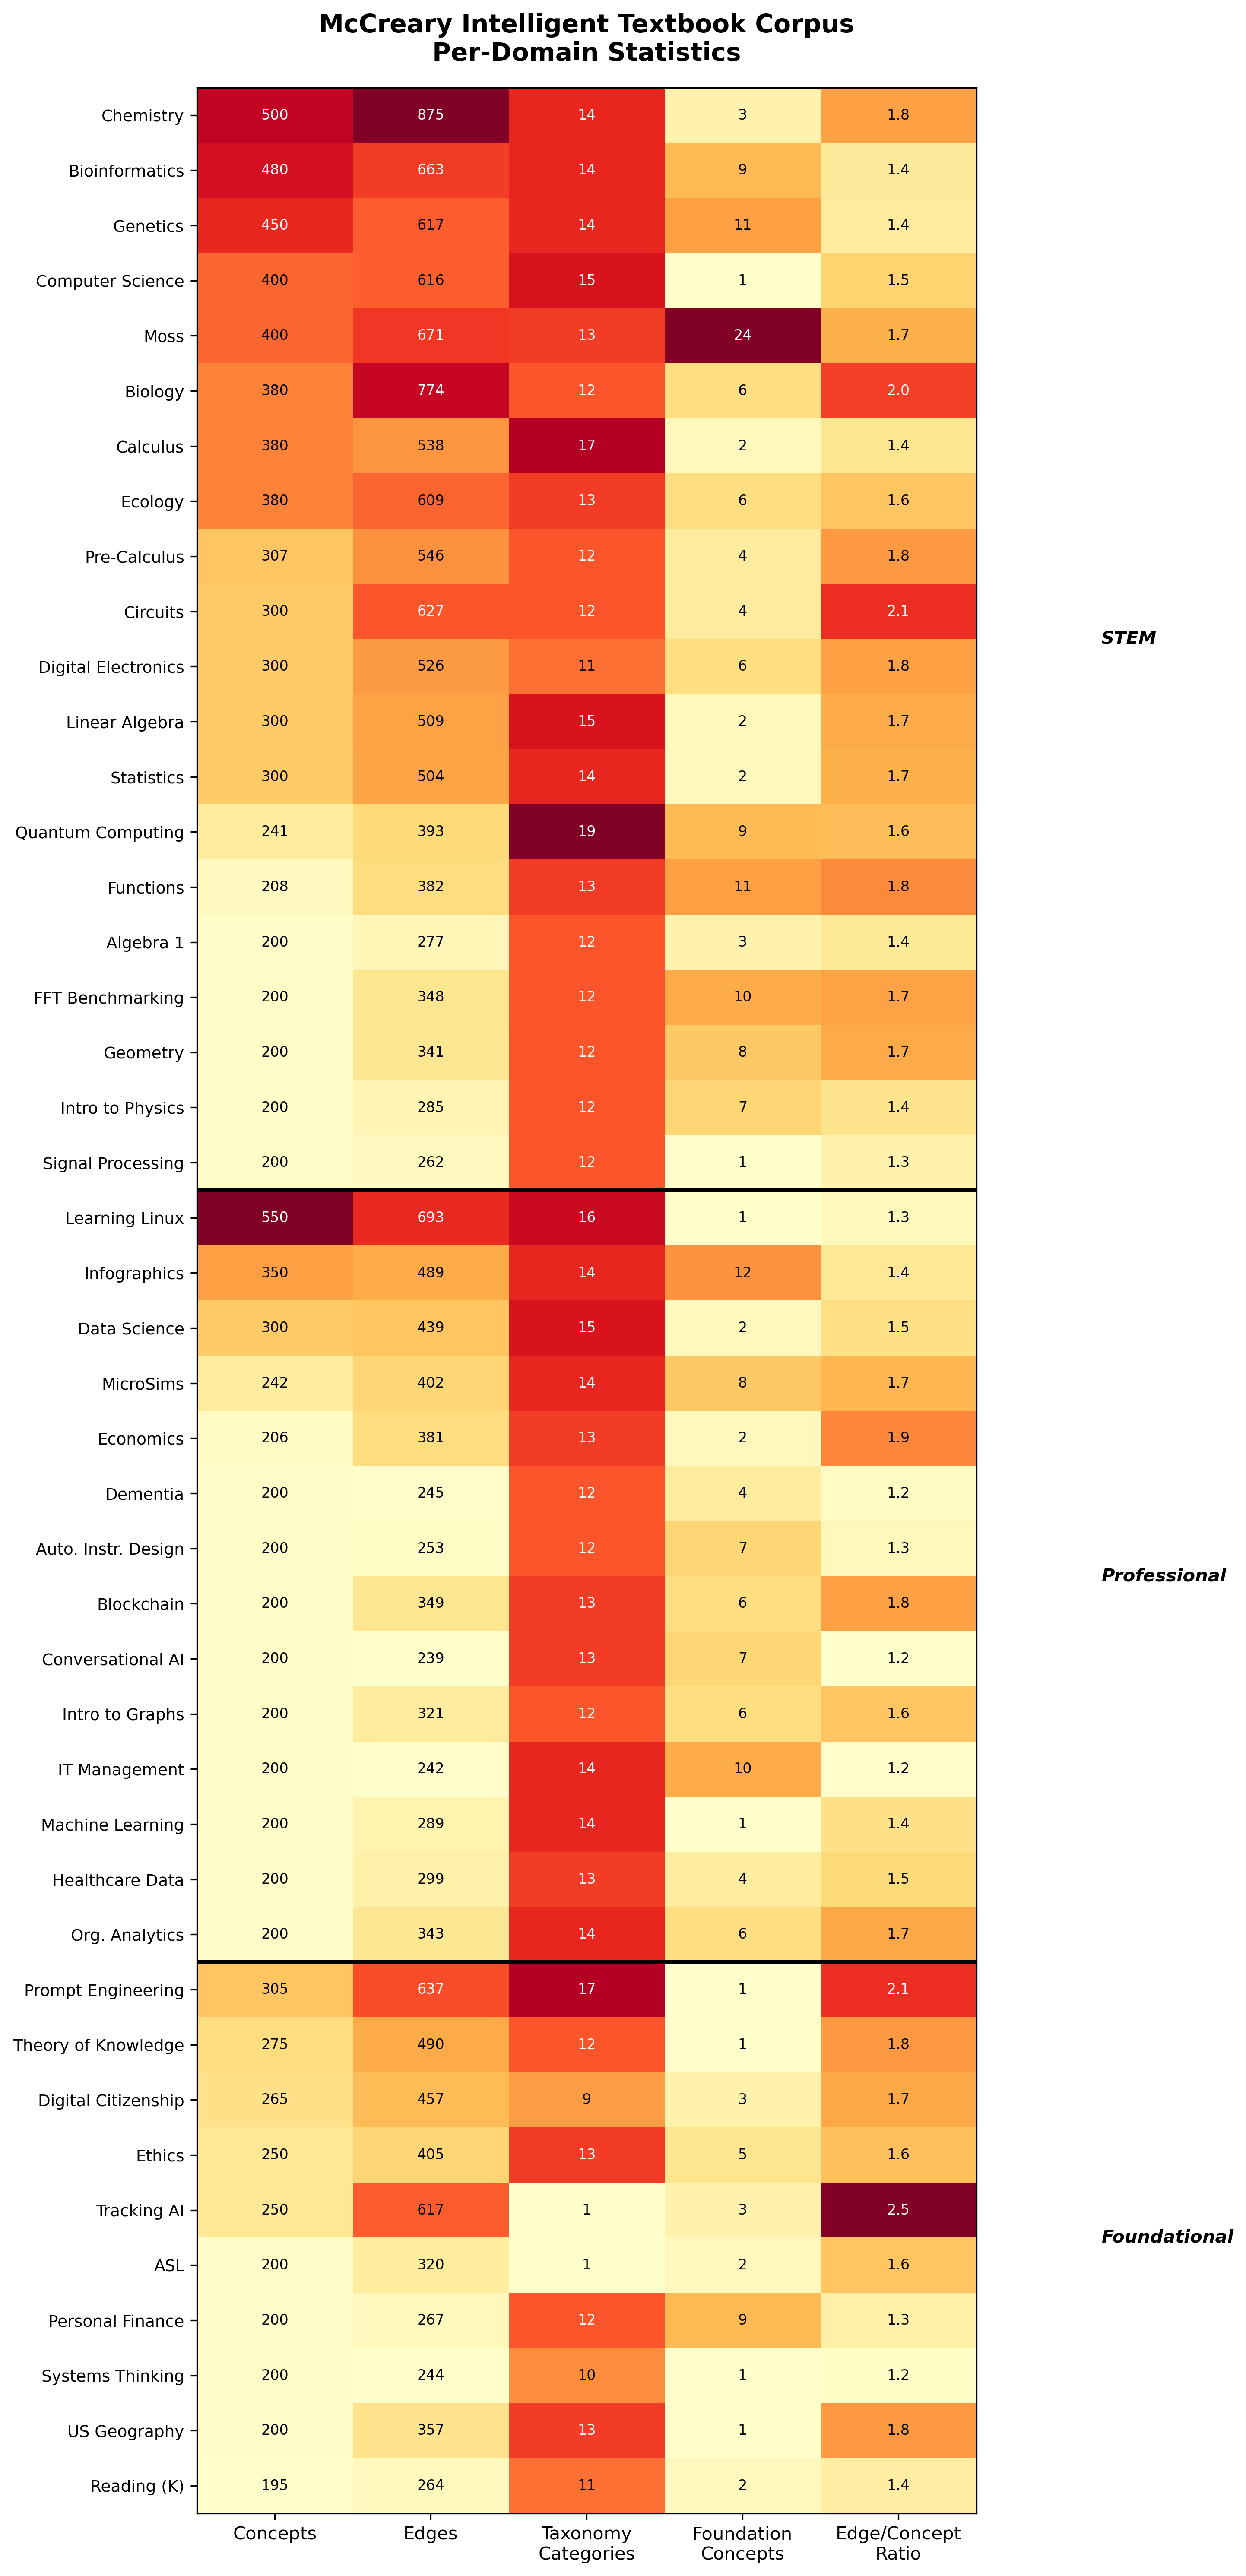
\includegraphics[width=0.95\textwidth]{figures/corpus-heatmap.png}
\caption{Per-domain statistics for the McCreary Intelligent Textbook Corpus.
Domains are grouped by category (STEM, Professional, Foundational) and sorted
by concept count. Color intensity reflects relative magnitude within each column.
Total: 12,260 concepts and 19,405 dependency edges across 46 domains.}
\label{fig:corpus-heatmap}
\end{figure}
